\documentclass{article}


% if you need to pass options to natbib, use, e.g.:
%     \PassOptionsToPackage{numbers, compress}{natbib}
% before loading neurips_2023


% ready for submission
\usepackage[final]{neurips_2023}


% to compile a preprint version, e.g., for submission to arXiv, add add the
% [preprint] option:
%     \usepackage[preprint]{neurips_2023}


% to compile a camera-ready version, add the [final] option, e.g.:
%     \usepackage[final]{neurips_2023}


% to avoid loading the natbib package, add option nonatbib:
%    \usepackage[nonatbib]{neurips_2023}


\usepackage[utf8]{inputenc} % allow utf-8 input
\usepackage[T1]{fontenc}    % use 8-bit T1 fonts
\usepackage{hyperref}       % hyperlinks
\usepackage{url}            % simple URL typesetting
\usepackage{booktabs}       % professional-quality tables
\usepackage{amsfonts}       % blackboard math symbols
\usepackage{nicefrac}       % compact symbols for 1/2, etc.
\usepackage{microtype}      % microtypography
\usepackage{xcolor}         % colors

\usepackage[pdftex]{graphicx}
\graphicspath{{./graphs/}}

\title{Procesamiento de imágenes (pre TP1)}

\author{
  Víctor A.~Bettachini\\ %\thanks{Use footnote for providing further information about author (webpage, alternative address)---\emph{not} for acknowledging funding agencies.} \\
  Datamining en ciencia y tecnología 2023\\
  Especialización en Explotación de Datos y Descubrimiento del Conocimiento\\
  \texttt{bettachini@gmail.com}
}


\begin{document}


\maketitle


\begin{abstract}
Cuca.
\end{abstract}


\section{Introducción}



\section{Materiales y métodos}

\paragraph{Datos}
210 imágenes de flores acompañados de un listado de las correspondientes especies dentro de una variedad de 10.
Las imágenes en formato png tienen una dimensión de 128 x 128 píxeles con tres canales de color.
El conjunto se descargó de una fuente pública [2].


\paragraph{Recurso informático} 
Un cuaderno (notebook) Jupyter provisto por los docentes en el sitio web denominado ``Campus'' [1] es la plantilla donde se escribió código en lenguaje Python.
Este explotó funciones de las bibliotecas OpenCV (\verb'cv2') y Clustimage para el trabajo con imágenes.
% Se modificó el sendero a los archivos para indicar un directorio en un sistema de archivos local de una computadora local para ejecutarle con mayor velocidad.


\section{Resultados}

\subsection{Preprocesamiento de los datos}
% Cada actividad realizada se describe bajo los titulos que figuran en el enunciado del trabajo práctico publicado en el

% Cargar el dataset y sus respectivas etiquetas. Es importante asegurarse que las imágenes sean comparables en color, valor, rango y tamaño.

% Explorar y graficar los subconjuntos de imágenes que representan flores de la misma especie



\subsection{Manipulación de datos}

% Cambiar la intensidad de una de las imágenes en escala de grises, transformarla en una imagen con mucho y otra con poco brillo.
\paragraph{Escala de grises}
Conocido el orden en que la función \verb'cv2.imread' carga los canales es azúl, verde, rojo (BGR: blue, green, red), se utilizó la combinación lineal que preserva la luminancia perceptual de la codificación de color sRGB de la Commission Internationale de l'éclairage en 1931 según el consorcio W3 \cite{cosa}, $
Y_\mathrm{lineal} = 0.2126 R_\mathrm{lineal} + 0.7152 G_\mathrm{lineal} + 0.0722 B_\mathrm{lineal} .
$

\paragraph{Brillo}
En la documentación de OpenCV [cosa] se indica que el ajuste de contraste y brillo se realiza con una función lineal
$
Y_\mathrm{lineal final} = \alpha Y_\mathrm{lineal inicial} + \beta ,
$
donde $\alpha$ la ganancia controla el contraste y $\beta$ el sesgo controla el brillo.

% Convertir una de las imágenes a blanco y negro (binario). ¿Es la única manera? Si existen otras transformaciones mostrar más de una conversión.

% Recortar una parte significativa de la imagen, quedándose sólo con el círculo central de la misma.

% Generar dos imágenes random: una imagen mezclando los pixels y otra mezclando partes de diferentes imágenes.

% Aplicar dos tipos diferentes de filtros sobre una imagen, explique en qué casos conviene usar cada uno.

% Calcular imagen promedio global y el promedio entre las distintas especies. ¿Se pueden distinguir los promedios? ¿Cómo quedan los promedios si consideran las imágenes en blanco y negro?

\subsection{Búsqueda de \emph{features}}

% Analizar las distribuciones de valores de pixels por cada especie. ¿Se puede distinguir una especie en algún rango de color?

% Realizar una inspección de las componentes principales del dataset y analizar si se pueden identificar las especies en esta representación.

\paragraph{Análisis de componentes principales}
Una centena de componentes principales por imagen se obtuvieron con el método \verb'exctract_feat' [3].


\section{Discusión}

\begin{figure}
  \centering
  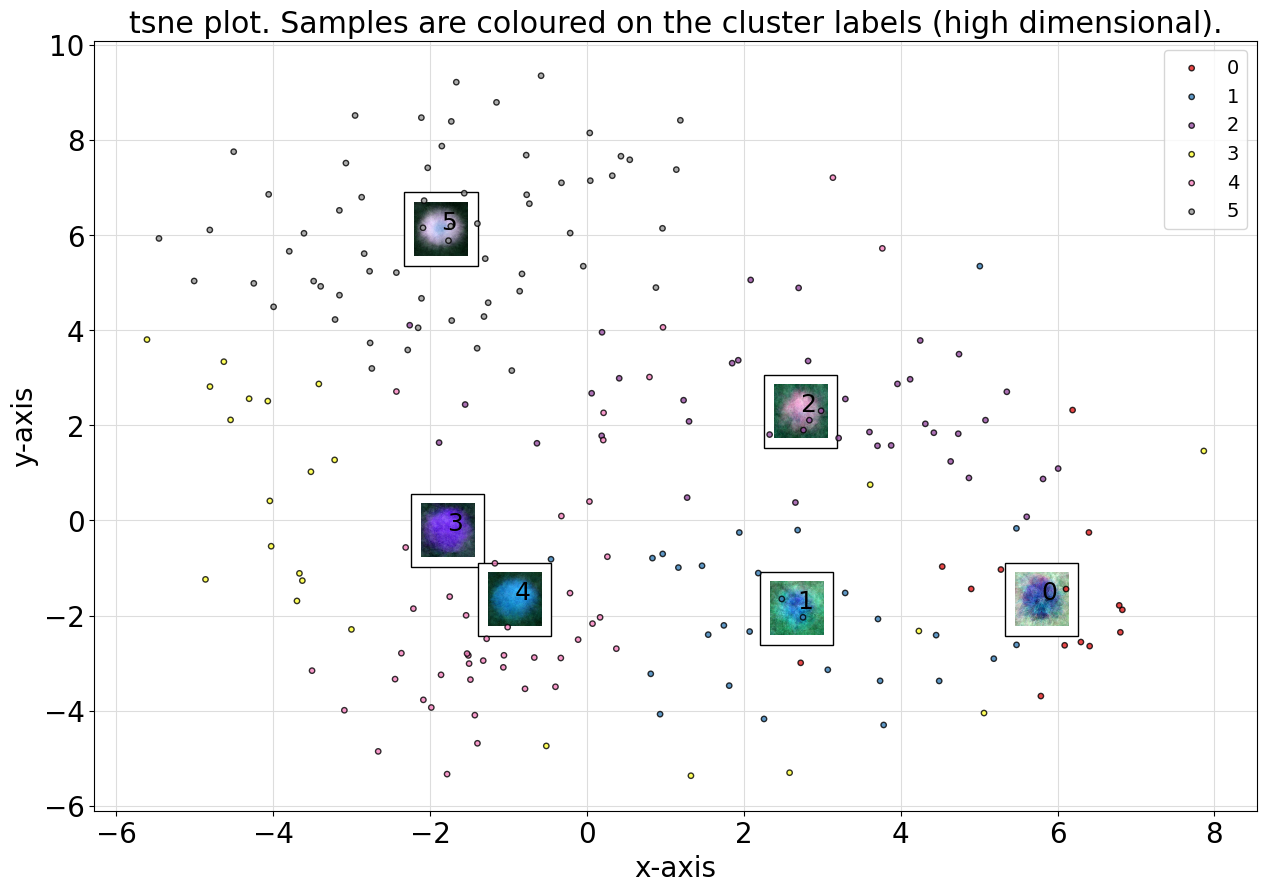
\includegraphics[width= 0.8\linewidth]{tsne}
  \caption{Ubicación de cada imágen en componentes principales(tsne plot)}
\end{figure}

\section*{References}

\medskip
{
\small

[1] Kamienkowski, J.A.\ \& \emph{et al.} (2023) {\it Campus de Datamining en ciencia y tecnología}, \url{https://datamining.dc.uba.ar/campus/course/view.php?id=37}

[2] Olga Belitskaya (2020, última actualización) Flower Color Images, {\it Kaggle}, \url{https://www.kaggle.com/olgabelitskaya/flower-color-images}

[3] Taskesen, E. (2020) PCA, {\it clustimage's documentation!}, \url{https://erdogant.github.io/clustimage/pages/html/Feature%20Extraction.html}
}

[4] Changing the contrast and brightness of an image \url{https://docs.opencv.org/3.4/d3/dc1/tutorial_basic_linear_transform.html} 
%%%%%%%%%%%%%%%%%%%%%%%%%%%%%%%%%%%%%%%%%%%%%%%%%%%%%%%%%%%%
% \bibliographystyle{unsrt}
% \bibliography{bibliography}
\begin{thebibliography}{9}
\bibitem{cosa}
Stokes, Michael; Anderson, Matthew; Chandrasekar, Srinivasan; Motta, Ricardo (1996-11-05). "A Standard Default Color Space for the Internet – sRGB". World Wide Web Consortium – Graphics on the Web. Part 2, matrix in equation 1.8. Archived from the original on 2023-05-24.
  \url{https://www.w3.org/Graphics/Color/sRGB}
\end{thebibliography}


  \end{document}